\section{The TP Problem}\label{sec:preliminTimelines}

As in the previous chapters, let $\Nat$ be the set of natural numbers and $\RealP$ be the set of non-negative real numbers; moreover, $\Intv$ denotes the set of intervals of $\RealP$ whose endpoints are in $\Nat\cup\{\infty\}$, and $\Intv_{(0,\infty)}$ is the set of non-singular%
\footnote{An interval of the form $[a,a]$, for $a\in\Nat$, is called \emph{singular}.} 
intervals $I\in \Intv$ such that
  either $I$ is unbounded, or $I$
  is left-closed with left endpoint $0$. The latter intervals $I$ can be replaced by expressions of the form $\sim n$, for some $n\in\Nat$
  and $\sim\,\in\{<,\leq,>,\geq\}$.
%
% Let $w$ be a finite word over some alphabet. By $|w|$ we denote the length of $w$. For all  $0\leq i<|w|$,  $w(i)$ is
% the $i$-th letter of $w$.


%\subsection{}\label{sec:timelines}

We now introduce notation and basic notions of
the TP framework as presented in~\cite{MayerOU16,GiganteMCO16}.
%
In TP, domain knowledge is encoded by a set of state variables, whose behaviour over time is described by transition functions and synchronization rules.

\begin{definition}[State variable]
  \label{def:statevar}
  A \emph{state variable} $x$ is a triple \[x= (V_x,T_x,D_x),\] where 
  \begin{itemize}
      \item $V_x$ is the \emph{finite domain} of the state variable $x$,
      \item $T_x:V_x\to 2^{V_x}$ is the \emph{value transition function}, which maps
        each $v\in V_x$ to the (possibly empty) set of successor values, and
      \item $D_x:V_x\to \Intv$ is the \emph{constraint (or duration) function} that maps each $v\in V_x$
        to an interval of $\Intv$.
  \end{itemize}   
\end{definition}

A \emph{token} for a variable $x$ is a pair $(v,d)$ consisting of a value $v\in V_x$ and a duration $d\in \RealP$
such that $d\in D_x(v)$. Intuitively, a token for $x$ represents an interval of time where the state variable $x$ takes value $v$.
In order to clarify the variable to which a token refers, we shall often denote $(v,d)$ as $(x,v,d)$.

The behavior of the state variable $x$ is specified by means of a \emph{timeline}, which is a non-empty sequence of tokens
$\pi = (v_0,d_0)\cdots  (v_n,d_n)$  consistent with the value transition function $T_x$, namely, such that
$v_{i+1}\in T_x(v_i)$ for all $0\leq i<n$. The \emph{start time} $\start(\pi,i)$ and the \emph{end time} $\Ending(\pi,i)$ of the $i$-th token of the timeline
$\pi$  are defined respectively as follows: 
\[\start(\pi,i)=0 \text{ if } i=0, \qquad \start(\pi,i)=\sum_{h=0}^{i-1} d_h \text{ otherwise},\]
and
\[\Ending(\pi,i)=\sum_{h=0}^{i} d_h.\]
%
See Figure~\ref{fig:timelineEx} for an example.
\begin{figure}
    \centering
    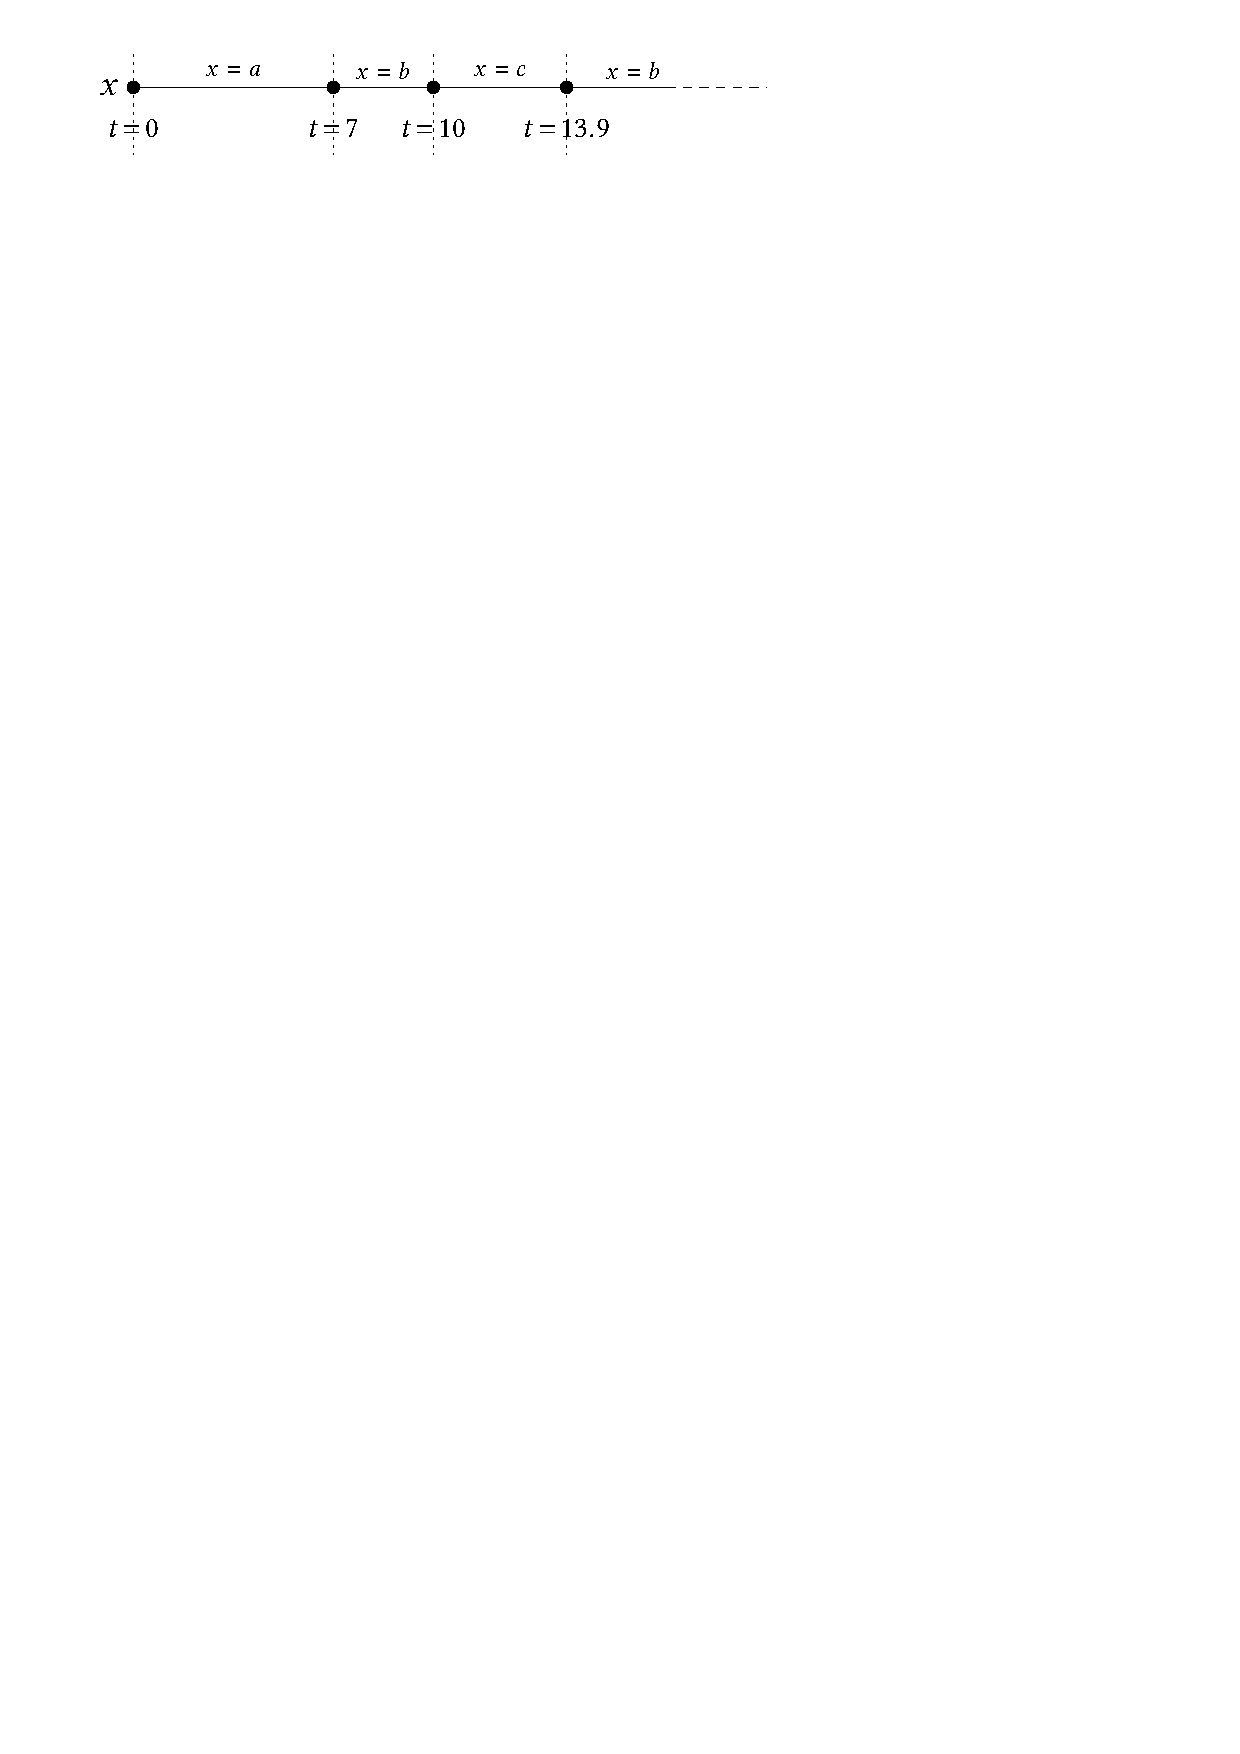
\includegraphics[scale=0.7]{Chaps/Timelines/timelineFig0.pdf}
    \caption{An example of timeline $(a,7)(b,3)(c,3.9)\cdots$ for the state variable $x= (V_x,T_x,D_x)$, where $V_x=\{a,b,c,\ldots\}$, $b\in T_x(a)$, $c\in T_x(b)$, $b\in T_x(c)$\dots\ and $D_x(a)=[5,8]$, $D_x(b)=[1,4]$, $D_x(c)=[2,\infty[$\dots}
    \label{fig:timelineEx}
\end{figure}

Given a finite set $SV$ of state variables, a \emph{multi-timeline} of $SV$ is a mapping $\Pi$ assigning to
each state variable $x\in SV$ a timeline for $x$.

Multi-timelines of $SV$ can be constrained by a set of \emph{synchronization
rules}, which relate tokens, possibly belonging to different timelines, through
temporal constraints on the start/end times of tokens (time-point constraints) and on the difference
between start/end times of tokens (interval constraints). The synchronization rules exploit
an alphabet $\Sigma=\{o,o_0,o_1,o_2,\ldots\}$ of token names to refer to the tokens along a multi-timeline, and are based on the notions of
\emph{atom} and \emph{existential statement}.

\begin{definition}[Atom]
  \label{def:timelines:atom}
  An \emph{atom} $\rho$ is either a clause of the form \mbox{$o_1\leq^{e_1,e_2}_{I} o_2$}
  (\emph{interval atom}), or of the forms $o_1\leq^{e_1}_{I} n$ or  $n\leq^{e_1}_{I}
  o_1$ (\emph{time-point atom}), where $o_1,o_2\in\Sigma$, $I\in\Intv$, $n\in\Nat$, and $e_1,e_2\in\{\start,\Ending\}$.
\end{definition}

An atom $\rho$ is evaluated with respect to a \emph{$\Sigma$-assignment $\lambda_\Pi$} for a given multi-timeline $\Pi$,
which is a mapping assigning to each token name $o\in \Sigma$ a pair $\lambda_\Pi(o)=(\pi,i)$ such that $\pi$ is a timeline of $\Pi$ and $0\leq i<|\pi|$ is a position along $\pi$ (intuitively,
$(\pi,i)$ represents the token of $\Pi$ referenced by the name $o$).

An interval atom $o_1\leq^{e_1,e_2}_{I} o_2$  \emph{is satisfied by  $\lambda_\Pi$} if $e_2(\lambda_\Pi(o_2))-e_1(\lambda_\Pi(o_1))\in I$.
A point atom $o\leq^{e}_{I} n$  (respectively, $n\leq^{e}_{I}o$)   \emph{is satisfied by  $\lambda_\Pi$} if $n-e(\lambda_\Pi(o))\in I$ (respectively, $e(\lambda_\Pi(o))-n\in I$).

\begin{definition}[Existential statement]
 An \emph{existential statement} $\mathcal{E}$ for a finite set $SV$ of state variables is a statement of the form
\[
\mathcal{E}=  \exists o_1[x_1=v_1]\cdots \exists o_n[x_n=v_n].\mathcal{C},
\]
  where $\mathcal{C}$ %$\mathcal{C}=\rho_0\land\ldots\land\rho_m$
  is a conjunction of atoms,
  $o_i\!\in\!\Sigma$, $x_i\!\in\! SV$, $v_i\!\in\! V_{x_i}$, for
  $1\leq i\leq n$. 

The elements $o_i[x_i=v_i]$ are called
  \emph{quantifiers}. A token name used in $\mathcal{C}$, but not occurring in any
  quantifier, is said to be \emph{free}. 
\end{definition}

  Given a $\Sigma$-assignment $\lambda_\Pi$ for a multi-timeline $\Pi$ of $SV$,
  we say that \emph{$\lambda_\Pi$ is consistent with the existential statement $\mathcal{E}$} if, for each quantifier $o_i[x_i=v_i]$, we have
   $\lambda_\Pi(o_i)=(\pi,h)$, where $\pi=\Pi(x_i)$ and the $h$-th token of $\pi$ has value $v_i$. A multi-timeline $\Pi$ of $SV$ \emph{satisfies} $\mathcal{E}$
   if there exists a $\Sigma$-assignment $\lambda_\Pi$ for $\Pi$ consistent with $\mathcal{E}$ such that each atom in $\mathcal{C}$ is satisfied by
   $\lambda_\Pi$.

We can now introduce synchronization rules, which constrain tokens, possibly belonging to different timelines.
\begin{definition}[Synchronization rule]
  A \emph{synchronization rule} $\mathcal{R}$ for a finite set $SV$ of state variables is a rule of one of the forms
  \[
  o_0[x_0=v_0] \to \mathcal{E}_1\lor \mathcal{E}_2\lor \ldots \lor \mathcal{E}_k, \qquad
          \true \to \mathcal{E}_1\lor \mathcal{E}_2\lor \ldots \lor \mathcal{E}_k,
  \]
  where $o_0\in\Sigma$, $x_0\in SV$, $v_0\in V_{x_0}$, and $\mathcal{E}_1, \ldots, \mathcal{E}_k$
  are \emph{existential statements}. % where only $o_0$ may appear free.
  In rules of the first
  form (which are called \emph{trigger rules}), the quantifier $o_0[x_0=v_0]$ is called \emph{trigger}; we require that only $o_0$ may appear free in $\mathcal{E}_i$, for all $1\leq i\leq n$. In rules of the second form (\emph{trigger-less rules}), we require
  that no token name appears free.
  \newline
  A trigger rule $\mathcal{R}$ is \emph{simple} if, for each existential statement $\mathcal{E}$ of $\mathcal{R}$ and each token name $o$ distinct from the trigger, there is at most one \emph{interval atom}
  of $\mathcal{E}$ where $o$ occurs.
\end{definition}

Intuitively, the  trigger $o_0[x_0=v_0]$ acts as a universal quantifier, which
states that \emph{for all} the tokens of the timeline for
$x_0$, where $x_0$ takes the
value $v_0$, at least one of the existential statements $\mathcal{E}_i$ must be satisfied. 
As an example, \[o_0[x_0=v_0]\to \exists o_1[x_1=v_1].o_0\leq^{\mathsf{e},\mathsf{s}}_{[2,\infty[} o_1\] states that after \emph{every} token for $x_0$ with value $v_0$ there exists a token for $x_1$ with value $v_1$ \emph{starting} at least 2 time instants after the \emph{end} of the former.
Trigger-less rules simply assert the
satisfaction of some existential statement. The intuitive meaning of \emph{simple} trigger rules is that they disallow simultaneous comparisons of multiple time-events
 (start/end times of tokens) with a non-trigger reference time-event. 
 
 The semantics of synchronization rules is formally defined as follows.
\begin{definition}[Semantics of synchronization rules]\label{def:semanticsRules}
Let $\Pi$ be a multi-timeline of a set $SV$ of state variables.

Given a \emph{trigger-less rule} $\mathcal{R}$ of $SV$, \emph{$\Pi$ satisfies $\mathcal{R}$} if $\Pi$ satisfies some existential statement of $\mathcal{R}$.

Given a \emph{trigger rule} $\mathcal{R}$ of $SV$ with trigger $o_0[x_0=v_0]$, \emph{$\Pi$ satisfies   $\mathcal{R}$} if, for every position $i$ of the
 timeline $\pi=\Pi(x_0)$ for $x_0$ such that $\pi(i)=(v_0,d)$, there exists an existential statement $\mathcal{E}$ of $\mathcal{R}$  and a $\Sigma$-assignment
 $\lambda_\Pi$ for $\Pi$ consistent with $\mathcal{E}$ such that $\lambda_\Pi(o_0)= (\pi,i)$ and $\lambda_\Pi$ satisfies all the atoms of $\mathcal{E}$.
\end{definition}

In the paper, we shall also focus on a stronger notion of satisfaction of trigger rules, called \emph{satisfaction under the future semantics}: it requires that all non-trigger tokens selected by some quantifier
%in the selected existential statements compared with the trigger token
do not start \emph{strictly before} the start time of the trigger token.

\begin{definition}[Future semantics of trigger rules]\label{def:futurerules}
  A multi-timeline $\Pi$ of $SV$ satisfies a trigger rule \[\mathcal{R}= o_0[x_0=v_0] \to \mathcal{E}_1\vee \mathcal{E}_2\vee
  \ldots \vee \mathcal{E}_k\]   \emph{under the future semantics} if $\Pi$ satisfies the trigger rule obtained from
  $\mathcal{R}$ by replacing each existential statement \[\mathcal{E}_i=\exists o_1[x_1=v_1]\cdots \exists o_n[x_n=v_n].\mathcal{C}\]
  by \[\mathcal{E}_i'=\exists o_1[x_1=v_1]\cdots \exists o_n[x_n=v_n].\Big(\mathcal{C}\wedge  \bigwedge_{i=1}^{n} o_0\leq^{\start,\start}_{[0,+\infty[} o_i\Big).\]
\end{definition}

A \emph{TP domain} $P=(SV,R)$ is specified by a finite set $SV$ of state variables and
a finite set $R$ of synchronization rules for $SV$ modeling their admissible behaviors.
Trigger-less rules can be used to express initial, as well as intermediate conditions
and the goals of the problem, while trigger rules are much more powerful and useful, for instance, to specify invariants and response requirements. 

A \emph{plan for $P=(SV,R)$} is a  multi-timeline of $SV$ satisfying all the rules in $R$. A \emph{future plan for $P$} is defined in a similar way, but we require satisfaction under the future semantics of \emph{all} trigger rules.

In the next sections we will study the following decision problems:
\begin{description}
  \item[TP problem] Given a TP domain $P=(SV,R)$, is there a plan for $P$?
  \item[Future TP problem] Given a TP domain $P\!=\!(SV\!,R)$, is there a \emph{future} plan for $P$?
\end{description}
%
%\begin{definition}%[Planning problem]
%  \label{def:timelines:problem}
%  A timeline-based planning \emph{problem} is a pair $P=(SV,S)$, where $SV$ is
%  a set of state variables and $S$ is a set of synchronization rules involving
%  variables in $SV$.
%  A \emph{plan} for
%  $P$ is a set of timelines $\Pi$, one for each $x_i\in SV$, such
%  that all the synchronization rules in $S$ are satisfied by the set $\Gamma$
%  of all tokens involved in (any of) the timelines of $\Pi$.
%\end{definition}

Table~\ref{tab:complex} summarizes all the decidability and complexity results described in the following about the mentioned problems:
we will consider mixes of restrictions on TP involving trigger rules with future semantics, simple trigger rules, and intervals in atoms (of trigger rules) which are non-singular or in $\Intv_{(0,\infty)}$.

\begin{table}[t]
    \centering    
    \caption{Decidability and complexity of restrictions of the TP problem.}
    \label{tab:complex}
    \resizebox{\linewidth}{!}{
    \begin{tabular}{r|c|c}
    	%\hline 
    	& TP problem & Future TP problem \\ 
    	\hline 
    	Unrestricted & Undecidable & (Decidable?) Non-primitive recursive-hard \\ 
    	\hline 
    	Simple trigger rules & Undecidable & Decidable (non-primitive recursive) \\ 
    	\hline 
    	Simple trigger rules, & \multirow{2}{*}{?} & \multirow{2}{*}{$\EXPSPACE$-complete} \\ 
    	non-singular intervals & & \\
    	\hline 
    	Simple trigger rules, & \multirow{2}{*}{?} & \multirow{2}{*}{$\Psp$-complete} \\ 
    	intervals in $\Intv_{(0,\infty)}$ & & \\
    	\hline 
    	Trigger-less rules only & $\NP$-complete & // \\ 
    	%\hline 
    \end{tabular} 
    }
\end{table}
